\documentclass{beamer}

\mode<presentation>
{
  \setbeamertemplate{background canvas}[square]
  \pgfdeclareimage[width=6em,interpolate=true]{dsailogo}{../dsai-logo}
  \pgfdeclareimage[width=6em,interpolate=true]{erasmuslogo}{../erasmus-logo}
  \titlegraphic{\pgfuseimage{dsailogo} \hspace{0.2in} \pgfuseimage{erasmuslogo}}
  %\usetheme{default}
  \usetheme{Madrid}
  \usecolortheme{rose}
  \usefonttheme[onlysmall]{structurebold}
}

\usepackage{pgf,pgfarrows,pgfnodes,pgfautomata,pgfheaps,pgfshade}
\usepackage{amsmath,amssymb}
\usepackage{graphics}
\usepackage{ragged2e}
\usepackage{array}
\usepackage[latin1]{inputenc}
\usepackage{colortbl}
\usepackage[absolute,overlay]{textpos}
\setlength{\TPHorizModule}{30mm}
\setlength{\TPVertModule}{\TPHorizModule}
\textblockorigin{10mm}{10mm}
\usepackage[english]{babel}
\usepackage{listings}
\setbeamercovered{dynamic}

\AtBeginSection[]{
  \begin{frame}<beamer>
  \frametitle{Outline}
  \tableofcontents[currentsection]
  \end{frame}
}

\title[Machine Learning]{Machine Learning\\Deep Learning}
\author{dsai.asia}
\institute[]{Asian Data Science and Artificial Intelligence Master's Program}
\date{}

% My math definitions

\renewcommand{\vec}[1]{\boldsymbol{#1}}
\newcommand{\mat}[1]{\mathtt{#1}}
\newcommand{\ten}[1]{\mathcal{#1}}
\newcommand{\crossmat}[1]{\begin{bmatrix} #1 \end{bmatrix}_{\times}}
\newcommand{\nullsp}[1]{{\cal N}(#1)}
\newcommand{\class}[1]{{\cal C}_{#1}}
\def\Rset{\mathbb{R}}
\def\Pset{\mathbb{P}}
\DeclareMathOperator*{\argmax}{argmax}
\DeclareMathOperator*{\argmin}{argmin}
\DeclareMathOperator*{\sign}{sign}
\DeclareMathOperator*{\cov}{Cov}
\DeclareMathOperator*{\diag}{diag}
\def\norm{\mbox{$\cal{N}$}}

\newcommand{\stereotype}[1]{\guillemotleft{{#1}}\guillemotright}

\newcommand{\myfig}[3]{\centerline{\includegraphics[width={#1}]{{#2}}}
    \centerline{\scriptsize #3}}

\begin{document}

%%%%%%%%%%%%%%%%%%%%%%%%%%%%%%%%%%%%%%%%%%%%%%%%%%%%%%%%%%%%
%%             CONTENTS START HERE

%\setbeamertemplate{navigation symbols}{}

\frame{\titlepage}

%--------------------------------------------------------------------
%\part<presentation>{Part name}
%
%\frame{\partpage}

\begin{frame}
\frametitle{Readings}

Readings for these lecture notes:
\begin{itemize}
\item[-] Goodfellow, I., Bengio, Y., and Courville, A. (2016),
  \textit{Deep Learning}, MIT Press, Chapter 6.
\item[-] Bishop, C. (2006), \textit{Pattern Recognition and Machine Learning},
  Springer, Chapters 3, 4, 6, 7.
\item[-] Hastie, T., Tibshirani, R., and Friedman, J. (2016),
  \textit{Elements of Statistical Learning: Data Mining, Inference, and
    Prediction}, Springer, Chapters 2, 3, 4, 12.
\item[-] Ng, A. (2017), \textit{Deep Learning},
  Lecture note set for CS229, Stanford University.
\end{itemize}

These notes contain material $\copyright$ Bishop (2006), Hastie et
al.\ (2016), Goodfellow et al.\ (2016), and Ng (2017).

\end{frame}

%======================================================================
\section{Introduction}
%======================================================================

\begin{frame}[fragile]
\frametitle{Introduction}

  Deep learning involves the training of so-called \alert{neural
    networks}.

  \medskip

  In this unit, we'll study how neural networks work and understand
  basic neural network learning algorithms.

  \medskip

  Then we'll briefly cover some of the modern neural network
  architectures that are generating so much layperson interest in AI
  today.

\end{frame}

%======================================================================
\section{Neural network intuition}
%======================================================================

\begin{frame}{Neural network intuition}{Basic units}

  To begin with, we'll consider the univariate regression setting
  where we want to learn a function $f : x \mapsto y$.

  \medskip

  A simple neural network can represent $f(x)$ by a single
  \alert{neuron} or \alert{unit} that computes
  \[ f(x) = \max(ax+b,0) \]
  for some fixed coefficients $a$ and $b$.

  \medskip

  This particular unit
  is called a \alert{ReLU} (rectified linear unit).

\end{frame}


\begin{frame}{Neural network intuition}{Composing units into networks}

  By stacking such units so that one passes its output to another, we can
  model increasingly complex functions.

  \medskip

  From Ng's course notes, consider the example in which we want to
  predict \alert{house price} given size, number of bedrooms, postal
  code, and wealth of the neighborhood the house is in.

  \medskip

  We could build the model up incrementally, having it compute
  a ``family size'' variable based on the house size and number of bedrooms.

  \medskip

  The postal code could be used to compute how ``walkable'' the neighborhood
  is.

  \medskip

  Combining the zip code with neighborhood wealth might predict
  ``school quality.''

\end{frame}


\begin{frame}{Neural network intuition}{Composing units into networks}

  We might finally decide that the price depends on these three derived
  features: family size, walkable, and school quality:

  \medskip

  \myfig{2.5in}{ng-nn}{Ng (2017), CS229 deep learning lecture notes.}

\end{frame}


\begin{frame}{Neural network intuition}{Composing units into networks}

  Another example: \alert{loan application underwriting}.

  \medskip

  One important attribute of a loan applicant is his/her \alert{income}.

  \medskip

  But high income is meaningless if the applicant's \alert{debt} is very
  high.

  \medskip

  Loan underwriters combine these two features into a higher level feature,
  \alert{debt-to-income ratio}.

  \medskip

  43\% is considered a ``magic'' tolerable debt-to-income ratio for a family.

\end{frame}


\begin{frame}{Neural network intuition}{End-to-end learning}

  See any problems with this architecture as we described it so far?

  \medskip

  Luckily, we don't need to solve those problems, as neural network
  learning is \alert{end-to-end learning}.

  \medskip

  That means \alert{the network figures out for itself what
    intermediate features are best for the task at hand}.

\end{frame}


\begin{frame}{Neural network intuition}{Hidden units}

  Intermediate units between the raw inputs and the output
  are called \alert{hidden units}.

  \medskip

  Example suppose we have:
  \begin{itemize}
  \item Four inputs $x_1$, $x_2$, $x_3$, and $x_4$
  \item Three hidden units
  \item A single output $y$
  \end{itemize}

  \medskip
  
  The goal of the network will be to \alert{find} intermediate
  features that will \alert{best predict} each $y^{(i)}$ from the
  corresponding $\vec{x}^{(i)}$.

  \medskip

  It may be difficult to understand the ``meaning'' of the intermediate
  features thus induced.

  \medskip

  Neural networks are therefore some times called \alert{black boxes}.

\end{frame}


\begin{frame}{Neural network intuition}{Some terminology}

  Here are the terms we've seen so far, and some new ones:
  \begin{itemize}
  \item A \alert{neuron} or \alert{unit} applies some function to its
    inputs to generate an output.
  \item Units may be composed into \alert{neural networks}.
  \item Input features are sometimes represented by units called
    \alert{input units} organized into a \alert{input layer}.
  \item One or more outputs comprise the \alert{output layer}.
  \item Intermediate units are called \alert{hidden units} and may be
    organized into zero or more \alert{hidden layers}.
  \end{itemize}

\end{frame}


\begin{frame}{Neural network intuition}{Notation}

  Suppose we have an input layer composed of features $x_1, x_2, \ldots$

  \medskip

  Ng uses the notation $a_i^{[j]}$ to indicate the \alert{activation}
  of the $i$th unit in the $j$th layer.

  \medskip

  $a_1^{[1]}$ is the output of the first hidden unit in the first hidden layer.

  \medskip

  $a_1^{[2]}$ is the output of the first unit in the second layer
  (the output layer in a network with only one hidden layer).

  \medskip

  To unify the notation, we let $a_i^{[0]} = x_i$, i.e., we treat
  the input as layer 0.

\end{frame}


\begin{frame}{Neural network intuition}{Activation functions}

  We saw a simple ReLU network already.

  \medskip

  \alert{Logistic regression} can also be treated as a simple neural network
  with one output unit and no hidden units:
  \[ g(\vec{x}) = \frac{1}{1+e^{-\vec{w}^\top\vec{x}}} \]
  is written in standard neural network notation as two steps:
  \begin{enumerate}
  \item Calculate the \alert{linear response} $z = \vec{w}^\top\vec{x}+b$.
  \item Calculate the \alert{activation function} $a = \sigma(z)$ where
    $\sigma(z) = 1 / (1+e^{-z})$.
  \end{enumerate}

\end{frame}


\begin{frame}{Neural network intuition}{Activation functions}

  Usually, $g(z)$ is nonlinear. The most common activation functions:
  \begin{itemize}
  \item The sigmoid $g(z) = \frac{1}{1+e^{-z}}$
  \item ReLU (the default activation function in modern neural
    networks) $g(z) = \max(z,0)$
  \item Hyperbolic tangent $g(z) = \frac{e^z-e^{-z}}{e^z+e^{-z}}$
  \end{itemize}

\end{frame}


\begin{frame}{Neural network intuition}{Full calculation}

  The full calculation proceeds as follows.

  \medskip

  For the first hidden unit in the
  first hidden layer, we calculate
  \[ z_1^{[1]} = \mat{W}_1^{[1]\top}\vec{x} + b_1^{[1]} \]
  and
  \[ a_1^{[1]} = g(z_1^{[1]}), \]
  where $\mat{W}$ is a matrix or parameters or weights.

  \medskip

  We repeat for each unit in each layer to get the final output
  layer.

\end{frame}


\begin{frame}{Neural network intuition}{What remains?}

  Now that we understand the feed-forward computation of a neural network,
  we'll talk about
  \begin{itemize}
  \item \alert{Efficient execution} of the feed-forward computation
  \item The \alert{gradient descent process} used to learn the weights
    $\mat{W}$.
  \end{itemize}
  
\end{frame}

%======================================================================
\section{Efficient computation}
%======================================================================

\begin{frame}{Efficient computation}{Calculating activations}

  Consider calculating hidden unit activations. We have
  $$\begin{matrix}
    z_1^{[1]} = \mat{W}_1^{[1]\top}\vec{x} + b_1^{[1]} & \text{and} & a_1^{[1]} = g(z_1^{[1]}) & \hfill \\
    \vdots & \vdots & \vdots & \hfill \\
    z_4^{[1]} = \mat{W}_4^{[1]\top}\vec{x} + b_4^{[1]} & \text{and} & a_4^{[1]} = g(z_4^{[1]}) & \hfill
  \end{matrix}$$

  Depending on the ``deepness'' of our model, for a single input, we
  may be doing an operation like this for hundreds or thousands of
  units.

  \medskip

  Code to implement this procedure using \texttt{for} loops and the
  like will run \alert{very slowly}, especially if implemented in a
  bytecode based language like Python or Java.

\end{frame}

  
\begin{frame}[fragile]{Efficient computation}{BLAS library}

  What is needed is the ability to perform matrix algebra with a
  single library call or instruction that is highly optimized, using
  CPU instructions provided for \alert{vector operations}.

  \medskip
  
  \alert{BLAS} is a well-known library that does this and is used by
  numpy:

\begin{tiny}
\begin{verbatim}
ldd /usr/lib/python3/dist-packages/numpy/core/multiarray.cpython-35m-x86_64-linux-gnu.so
	linux-vdso.so.1 =>  (0x00007fff40fde000)
	libblas.so.3 => /usr/lib/libblas.so.3 (0x00007f9a14579000)
	libm.so.6 => /lib/x86_64-linux-gnu/libm.so.6 (0x00007f9a14270000)
	libpthread.so.0 => /lib/x86_64-linux-gnu/libpthread.so.0 (0x00007f9a14053000)
	libc.so.6 => /lib/x86_64-linux-gnu/libc.so.6 (0x00007f9a13c89000)
	/lib64/ld-linux-x86-64.so.2 (0x00007f9a14b69000)
	libopenblas.so.0 => /usr/lib/libopenblas.so.0 (0x00007f9a11bf5000)
	libgfortran.so.3 => /usr/lib/x86_64-linux-gnu/libgfortran.so.3 (0x00007f9a118ca000)
	libquadmath.so.0 => /usr/lib/x86_64-linux-gnu/libquadmath.so.0 (0x00007f9a1168b000)
	libgcc_s.so.1 => /lib/x86_64-linux-gnu/libgcc_s.so.1 (0x00007f9a11475000)
\end{verbatim}
\end{tiny}

  \medskip

  Alternatively, we may parallelize computation by recruiting GPU resources.

\end{frame}

  
\begin{frame}[fragile]{Efficient computation}{Vectorized activation calculation}

  For an entire layer, to use vectorized computation, we need to perform
  the operation in one operation:

  \[ \vec{z}^{[1]} = \mat{W}^{[1]\top} \vec{x} + \vec{b}^{[1]} \]

  This can be implemented in a single Python statement:

\begin{verbatim}
W1 = np.matrix(np.random.normal(0,1,(3,4)))
b1 = np.matrix(np.random.normal(0,1,(4,1)))
x = np.matrix(np.random.normal(0,1,(3,1)))
z1 = W1.T * x + b1
\end{verbatim}

  This would run much faster than the equivalent doubly-nested
  \texttt{for} loop.

\end{frame}

  
\begin{frame}[fragile]{Efficient computation}{Vectorized activation calculation}

  Then to calculate $\vec{a}^{[1]}$ as a vector operation, we can
  hopefully use vectorized functions in our implementation language.

  \medskip

  If we have the sigmoid function, for example, we implement
  \[ g(z_i^{[1]}) = \frac{1}{1+e^{-z_i^{[1]}}} \]
  as
  \begin{verbatim}
def g(z):
    return 1 / (1 + exp(-z))
z = np.matrix([[1,2,3]]).T
a = g(z)
  \end{verbatim}

  This will run much faster than executing the \texttt{exp()} function
  within a Python loop.
  
\end{frame}

  
\begin{frame}[fragile]{Efficient computation}{Vectorizing over training examples}

  Next, consider performing a calculation over \alert{many training examples}.

  \medskip

  Performing the operation
  \[ \vec{z}^{[1]} = \mat{W}^{[1]\top} \vec{x}^{(i)} + \vec{b}^{[1]} \]
  inside a loop for every training example $i$ would be slower than the
  vectorized operation
  \[ \vec{z}^{[1]} = \mat{W}^{[1]\top} \mat{X}^\top + \vec{b}^{[1]}. \]
  Note: despite different dimensions of
  $\mat{W}^{[1]\top} \mat{X}^\top$ and $\vec{b}^{[1]}$,
  some languages like Python allow \alert{broadcasting} of the addition
  operation horizontally:
  \begin{verbatim}
>>> W = np.matrix([[1,2,3],[2,3,4]])
>>> b = np.matrix([[2,3]]).T
>>> W+b
matrix([[3, 4, 5],
        [5, 6, 7]])
\end{verbatim}  

\end{frame}

%======================================================================
\section{Backpropagation}
%======================================================================

\begin{frame}{Backpropagation}{Introduction}

  Now that we understand how the feedforward computation of a neural
  network works and how to use optimized vector operations, let's consider
  how to train a neural network.

  \medskip

  The general procedure is called \alert{backpropagation}.

  \medskip
  
  \begin{columns}

    \column{1.6in}
    
  \framebox{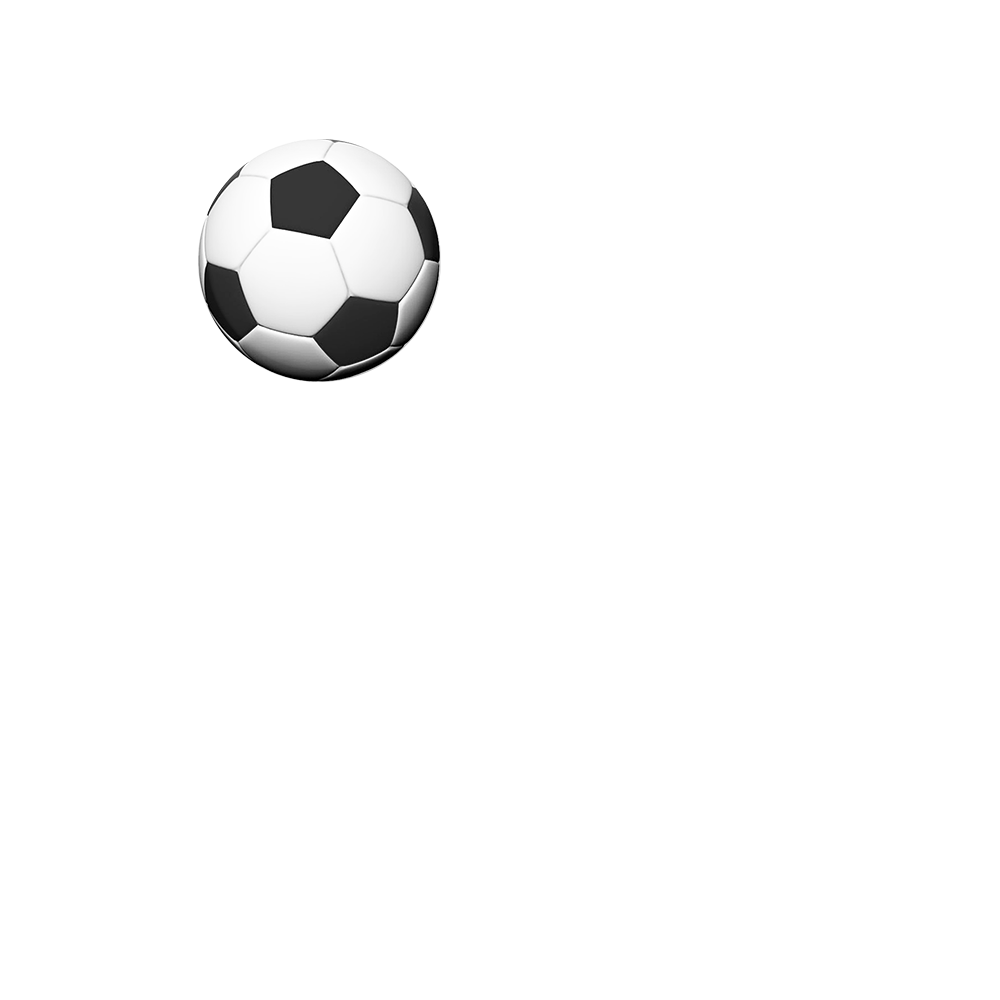
\includegraphics[width=1.5in]{soccer}}

  \column{2.9in}

  We'll use Ng's (2017) example of classifying an image as containing a
  soccer ball or not.

  \end{columns}
  
\end{frame}


\begin{frame}{Backpropagation}{Flattening the input}

  First we'll scale the image to a standard size, for example 64 $\times$ 64.

  \begin{center}    
    \framebox{
\includegraphics[width=0.75in]{soccer64}}
  \end{center}

  Then we'll \alert{flatten} the 64 $\times$ 64 $\times$ 3 elements
  of the input to a 12,288-element vector and present to our neural network:

  \medskip
  
  \myfig{3.5in}{soccer-flatten}{Ng (2017), CS 229 Lecture notes on deep learning}
  
\end{frame}


\begin{frame}{Backpropagation}{Model, architecture, parameters}

  Some terminology a neural network \alert{model} consists of
  \begin{itemize}
  \item The network \alert{architecture} (number of layers, units, type of units, connectivity between units),
  \item The \alert{parameters} (the values of the weights $\mat{W}^{[i]}$ and
    $\vec{b}^{[i]}$.
  \end{itemize}

  \medskip

  In the forthcoming analysis, we'll assume a 3-layer network architecture

  \myfig{2.5in}{three-layer}{Ng (2017), Deep learning lecture notes for CS 229.}

  The architecture consists of two \alert{fully connected layers}
  followed by a single \alert{logistic sigmoid output}. Now we
  consider how to learn the $3n+14$ parameters of the model through
  backpropagation.

\end{frame}


\begin{frame}{Backpropagation}{Parameter initialization}

  First step: \alert{set initial values of the parameters}.

  \medskip

  Initializing to 0 would be a bad idea, because the output of each layer
  would be identical for every unit, and the gradients backpropagated
  later would also be identical.

  \medskip

  Solution: randomly initialize parameters to small values close to 0,
  e.g., \[ w^{[i]}_{jk} \sim {\cal N}(0,0.1). \]

  A better method in practice is called Xavier/He initialization:
  \[ w^{[i]}_{jk} \sim {\cal N}\left(0,\sqrt{\frac{2}{n^{[i]}+n^{[i-1]}}} \right), \]
  where $n^{[i]}$ is the number of units in layer $i$. This encourages
  the variance of the outputs of a layer to be similar to the variance
  of the inputs.
  
\end{frame}


\begin{frame}{Backpropagation}{Parameter initialization}

  Note that for \alert{ReLU hidden units}, the recommendation for the
  \alert{bias weights} is to use a small \alert{positive} (even
  constant) initial value.

  \medskip

  This ensures that the unit's output is initially positive for most
  training examples.
  
\end{frame}


\begin{frame}{Backpropagation}{Parameter update}

  In the case of a single logistic sigmoid at the output layer, after
  forward propagation, we have a predicted value $\hat{y}$.

  \medskip

  Neural network parameter update rules are usually derived in terms of
  backpropagating an \alert{error} or \alert{loss}.

  \medskip

  If we have an objective function such as
  maximum likelihood, we can convert to a loss by \alert{negating} it.

  \medskip

  We thus get the \alert{log loss} function for a network with a single
  logistic sigmoid output:
  \[ {\cal L}(\hat{y},y) = - \left[(1-y)\log(1-\hat{y})+y\log\hat{y}\right]. \]

  Note that it is easy to do the same for a linear output (Gaussian
  distribution for $y$) or softmax ouptut (multinomial distribution
  for $y$).\footnote{See Goodfellow et al.\ (2016) Section 6.2.2.4 for
    discussion of other output types.}

\end{frame}


\begin{frame}{Backpropagation}{Parameter update}

  Now, to update the parameters in layer $l$, we update using
  \alert{gradient descent} on the log loss:
  \begin{eqnarray*}
    \mat{W}^{[l]} & \leftarrow & \mat{W}^{[l]} - \alpha \frac{\partial {\cal L}}{\partial \mat{W}^{[l]}} \\
    \vec{b}^{[l]} & \leftarrow & \vec{b}^{[l]} - \alpha \frac{\partial {\cal L}}{\partial \vec{b}^{[l]}}
  \end{eqnarray*}
  
\end{frame}


\begin{frame}{Backpropagation}{Parameter update}

  First we consider the weights at the output layer. We have
  \begin{eqnarray*}
    \frac{\partial {\cal L}}{\partial \mat{W}^{[3]}} & = &
    - \frac{\partial}{\partial \mat{W}^{[3]}} \left( (1-y)\log(1-\hat{y})+y \log \hat{y} \right) \\
    & = & -(1-y)\frac{\partial}{\partial \mat{W}^{[3]}} \log
    \left( 1 - g(\mat{W}^{[3]}\vec{a}^{[2]} + \vec{b}^{[3]}) \right) \\
    & & \;\;\;\;\; - y \frac{\partial}{\partial \mat{W}^{[3]}} \log \left(
    g(\mat{W}^{[3]}\vec{a}^{[2]} + \vec{b}^{[3]} ) \right) \\
    & = & \frac{(1-y)g'(\mat{W}^{[3]}\vec{a}^{[2]} + \vec{b}^{[3]})\vec{a}^{[2]\top}}{1 - g(\mat{W}^{[3]}\vec{a}^{[2]} + \vec{b}^{[3]})} \\
    & & \;\;\;\;\; -\frac{y g'(\mat{W}^{[3]}\vec{a}^{[2]} + \vec{b}^{[3]})\vec{a}^{[2]\top}}{g(\mat{W}^{[3]}\vec{a}^{[2]} + \vec{b}^{[3]} )}
  \end{eqnarray*}

\end{frame}


\begin{frame}{Backpropagation}{Parameter update}

  Continuing, we note that for this model, $g(z)$ is the logistic
  sigmoid.

  \medskip

  Let's replace $g(z)$ with $\sigma(z)$ and $g'(z)$ with
  $\sigma'(z)$ to make this clear.

  \medskip

  We also recall that $\sigma'(z) = \sigma(z)(1-\sigma(z))$, allowing
  us to simplify the expression:
  \begin{eqnarray*}
    \frac{\partial {\cal L}}{\partial \mat{W}^{[3]}} & = & ... \\
    & = & (1-y)\sigma(\mat{W}^{[3]}\vec{a}^{[2]} + \vec{b}^{[3]})\vec{a}^{[2]\top}    -y (1-\sigma(\mat{W}^{[3]}\vec{a}^{[2]} + \vec{b}^{[3]}))\vec{a}^{[2]\top}\\
    & = & (1-y)a^{[3]}\vec{a}^{[2]\top}-y (1-a^{[3]})\vec{a}^{[2]\top} \\
    & = & (a^{[3]}-y)\vec{a}^{[2]\top}.
  \end{eqnarray*}

\end{frame}


\begin{frame}{Backpropagation}{Parameter update}

  What about the weights for layer 2?

  \medskip

  We can use the chain rule from calculus. When we have a function $f(z)$
  where $z = g(x)$, we can write
  \[ \frac{\partial f}{\partial x} =
  \frac{\partial f}{\partial g}\frac{\partial g}{\partial x} \]
  In our case we have
  \[ \frac{\partial {\cal L}}{\partial \mat{W}^{[2]}} =
  \frac{\partial \cal L}{\partial a^{[3]}}
  \frac{\partial a^{[3]}}{\partial \vec{z}^{[3]}}
  \frac{\partial \vec{z}^{[3]}}{\partial \vec{a}^{[2]}}
  \frac{\partial \vec{a}^{[2]}}{\partial \vec{z}^{[2]}}
  \frac{\partial \vec{z}^{[2]}}{\partial \mat{W}^{[2]}} . \]
  
\end{frame}


\begin{frame}{Backpropagation}{Parameter update}

  To evaluate this expression, let's try to reuse what we already
  have for $\frac{\partial \cal L}{\partial \mat{W}^{[3]}}$ first:
  \[ \frac{\partial \cal L}{\partial \mat{W}^{[3]}} =
  \frac{\partial \cal L}{\partial a^{[3]}}
  \frac{\partial a^{[3]}}{\partial \vec{z}^{[3]}}
  \frac{\partial \vec{z}^{[3]}}{\partial \mat{W}^{[3]}} =
  (a^{[3]}-y)\vec{a}^{[2]} \]
  
  we can reuse the part
  \[ \frac{\partial \cal L}{\partial \vec{z}^{[3]}} = \frac{\partial \cal L}{\partial a^{[3]}}
  \frac{\partial a^{[3]}}{\partial \vec{z}^{[3]}} = 
  a^{[3]}-y. \]

  For the remaining terms, we have
  \begin{eqnarray*}
    \frac{\partial \vec{z}^{[3]}}{\partial \vec{a}^{[2]}} & = & \mat{W}^{[3]}\\
    \frac{\partial \vec{a}^{[2]}}{\partial \vec{z}^{[2]}} & = & g'(\vec{z}^{[2]})\\
    \frac{\partial \vec{z}^{[2]}}{\partial \mat{W}^{[2]}} & = & \vec{a}^{[1]}.
  \end{eqnarray*}
    
\end{frame}


\begin{frame}{Backpropagation}{Parameter update}

  Putting the chain rule terms together in an order appropriate for
  vector calculations, we obtain
  \[ \frac{\partial \cal L}{\partial \mat{W}^{[2]}} =
  \diag(g'(\vec{z}^{[2]}))
  \mat{W}^{[3]}
  (a^{[3]}-y)\vec{a}^{[1]\top}. \]

  \medskip
  
  The calculation is also similar for the bias weights, except that
  in place of $\vec{a}^{[1]}$ we have 1.

\end{frame}


\begin{frame}{Backpropagation}{Parameter update}

  What about the weights for \alert{layer 1}?

  \medskip
  
  We want
  \[ \frac{\partial \cal L}{\partial w^{[1]}_{ij}}. \]
  We can readily see that $w^{[1]}_{ij}$ affects \alert{all} of the
  second layer activations $\vec{a}^{[2]}$.

  \medskip

  In this case, the applicable more general chain rule,
  when $y = f(\vec{u})$ and $\vec{u} = g(\vec{x})$ is 
  \[ \frac{\partial y}{\partial x_i} = \sum_j \frac{\partial y}{\partial u_j}
  \frac{\partial u_j}{\partial x_i}. \]

\end{frame}


\begin{frame}{Backpropagation}{Parameter update}

  In our case, the generalized chain rule gives  
  \[ \frac{\partial \cal L}{\partial w^{[1]}_{ij}} = \sum_k
  \frac{\partial \cal L}{\partial a^{[2]}_k}
  \frac{\partial a^{[2]}_k}{\partial w^{[1]}_{ij}} . \]
  
  \medskip

  Expanding the two terms within the summation, we obtain
  \[ \frac{\partial \cal L}{\partial w^{[1]}_{ij}} = \sum_k
  \frac{\partial \cal L}{\partial a^{[3]}}
  \frac{\partial a^{[3]}}{\partial z^{[3]}}
  \frac{\partial z^{[3]}}{\partial a^{[2]}_k}
  \frac{\partial a^{[2]}_k}{\partial z^{[2]}_k}
  \frac{\partial z^{[2]}_k}{\partial a^{[1]}_j}
  \frac{\partial a^{[1]}_j}{\partial z^{[1]}_j}
  \frac{\partial z^{[1]}_j}{\partial w^{[1]}_{ij}} . \]
  
\end{frame}


\begin{frame}{Backpropagation}{Parameter update}

  Getting complicated, right?

  \medskip

  The key to solving the problem efficiently is realizing that the term
  \[ \frac{\partial \cal L}{\partial a^{[3]}}
  \frac{\partial a^{[3]}}{\partial z^{[3]}}
  \frac{\partial z^{[3]}}{\partial a^{[2]}_k}
  \frac{\partial a^{[2]}_k}{\partial z^{[2]}_k} \]
  has already been calculated, in the process of determining
  \[ \frac{\partial \cal L}{\partial w^{[2]}_{jk}} ! \]
  Really, go back and check.
  Now we see that we generally want to reuse terms that look like
  $\frac{\partial \cal L}{\partial z^{[l]}_i}$.

  \medskip
  
  Let's therefore define
  \[ \delta^{[l]}_i = \frac{\partial \cal L}{\partial z^{[l]}_i} .\]
  We then obtain the backpropagation algorithm for our sample network...


\end{frame}


\begin{frame}{Backpropagation}{Parameter update}

  \begin{tabbing}
    xxx \= xxx \= xxx \= \kill
    \underline{\textbf{Backpropagation (fully-connected network)}} \\
    Given example $(\vec{x},y)$:\\
    \> $\vec{a}^{[0]} \leftarrow \vec{x}.$ \\
    \> for $l = 1..L$ do \\
    \> \> $\vec{z}^{[l]} \leftarrow \mat{W}^{[l]} \vec{a}^{[l-1]} + \vec{b}^{[l]}.$ \\
    \> \> $\vec{a}^{[l]} \leftarrow g^{[l]}(\vec{z}^{[l]})$. \\
    \> $\vec{\delta}^{[L]} \leftarrow \frac{\partial \cal L}{\partial \vec{z}^{[L]}}.$ \\
    \> for $l = L..1$ do\\
    \> \> $\frac{\partial \cal L}{\partial \mat{W}^{[l]}} \leftarrow \vec{\delta}^{[l]} \vec{a}^{[l-1]\top}.$ \\
    \> \> $\frac{\partial \cal L}{\partial \vec{b}^{[l]}} \leftarrow \vec{\delta}^{[l]}$.\\
    \> \> if $l > 1$ then\\
    \> \> \> $\vec{\delta}^{[l-1]} \leftarrow
    \diag(g'(\vec{z}^{[l-1]}))
    \mat{W}^{[l]}
    \vec{\delta}^{[l]}$
  \end{tabbing}

\end{frame}


\begin{frame}{Backpropagation}{Stochastic vs.\ batch gradient descent}

  Thus far, the derviation was for a single $(\vec{x},y)$ pair.

  \medskip

  What about batch gradient descent? We would use the rule
  \[ \mat{W}^{[l]} \leftarrow \mat{W}^{[l]} - \alpha \frac{\partial J}{\partial \mat{W}^{[l]}}, \]
  where $J$ is the cost function
  \[ J = \frac{1}{m}\sum_{i=1}^m {\cal L}^{(i)} \]
  and ${\cal L}^{(i)}$ is the loss for a single example.

  \medskip

  Stochastic gradient descent will be more noisy but will usually
  converge faster than batch gradient descent.

\end{frame}


\begin{frame}{Backpropagation}{Mini-batch gradient descent}

  Since batch gradient descent is more accurate but slower to get
  moving than stochastic gradient descent, a common compromise is
  \alert{mini-batch gradient descent}.

  \medskip

  The mini-batch is a compromise between the accuracy of batch and the
  the speed of stochastic gradient descent. We split the data set into
  partitions $B_1, B_2, \ldots$ (or repeatedly sample uniformly from
  the full training set) and let
  \[ J_{i} = \frac{1}{|B_i|}\sum_{j \in B_i}{\cal L}^{(j)}. \]

\end{frame}


\begin{frame}{Backpropagation}{Momentum}

  Another common optimization is called \alert{momentum}.

  \medskip

  The problem is that sometimes noisy data make us jump back and forth across valleys in the loss function, leading to slow convergence.

  \medskip

  With momentum, we remember the last update to each parameter and use
  it to calculate a moving average of the gradient over time.

  \medskip

  We use the following update rule:
  \begin{eqnarray*}
    \mat{V}_{dW^{[l]}} & \leftarrow & \beta \mat{V}_{dW^{[l]}}+ (1-\beta)
    \frac{\partial J}{\partial \mat{W}^{[l]}} \\
    \mat{W}^{[l]} & \leftarrow & \mat{W}^{[l]} - \alpha \mat{V}_{dW^{[l]}}
  \end{eqnarray*}

  The momentum term $\beta$ will encourage the optimization to
  accelerate gradually toward the minimum.
    
\end{frame}


\begin{frame}{Backpropagation}{Adam optimization}

  For a more sophisticated version of momentum that is adaptive,
  take a look at the famous ICLR 2015 paper on \alert{Adam}:
  
  \medskip

  Kingma, D.P.\ and Ba, J.L.\ (2015), Adam: A Method for
  Stochastic Optimization. In \textit{International Conference on Learning
    Representations}.

  \medskip

  Adam usually outperforms other optimization methods such as SGD with
  momentum or RMSProp when applied to large NN models.

\end{frame}

%======================================================================
\section{Avoiding overfitting}
%======================================================================

\begin{frame}{Avoiding overfitting}{Overfitting}

  Neural networks are \alert{universal approximators}.

  \medskip

  Roughly speaking, given enough training data and sufficient model
  complexity, backpropgation can learn \alert{any function} to an
  arbitrary level of accuracy.

  \medskip

  But when model complexity is too high for the training set size, we
  observe \alert{overfitting}: training accuracy is high, but
  validation set/test set accuracy is substantially lower.

  \medskip

  Solutions:
  \begin{itemize}
  \item Decrease model complexity (remove hidden units, remove layers)
  \item Collect more training data
  \item Regularization
  \end{itemize}
  
\end{frame}


\begin{frame}{Avoiding overfitting}{Regularization}

  Let $\vec{w}$ denote a single vector containing the set of all
  parameters in our model (every $w^{[l]}_{ij}$ and $b^{[l]}_i$).

  \medskip

  Let $J$ be the model cost function.

  \medskip

  L2 regularization adds a new term to the cost function:
  \begin{eqnarray*}
    J_{L2} & = & J + \frac{\lambda}{2}\|\vec{w}\|^2 \\
    & = & J + \frac{\lambda}{2}\vec{w}^\top\vec{w}
  \end{eqnarray*}

  \medskip

  Why do this?
  \begin{itemize}
  \item $\lambda=0$ gives us unregularized parameter learning.
  \item Big $\lambda$ encourages solutions with small $\vec{w}$,
    especially, \alert{as many 0 elements as possible}.
  \end{itemize}

  Forcing less useful parameters to 0 decreases model complexity and
  will reduce overfitting.
  
\end{frame}


\begin{frame}{Avoiding overfitting}{Regularization}

  How does the regularizer affect the learning rule?

  \medskip

  Previously, we had
  \[ \vec{w} \leftarrow \vec{w} - \alpha \frac{\partial J}{\partial \vec{w}}. \]
  Now we have
  \begin{eqnarray*}
    \vec{w} & \leftarrow & \vec{w} - \alpha \frac{\partial J}{\partial \vec{w}} - \alpha \frac{\lambda}{2} \frac{\partial \vec{w}^\top\vec{w}}{\partial \vec{w}} \\
    & = & (1 - \alpha \lambda)\vec{w} - \alpha \frac{\partial J}{\partial \vec{w}}
  \end{eqnarray*}
  Think about what this means ($\alpha$ and $\lambda$ are both small
  positive reals).

  \medskip

  On each update, we make all the weights' magnitudes a little
  smaller. Only the most important weights will survive.
  
\end{frame}


\begin{frame}{Avoiding overfitting}{Parameter sharing}

  Let's return to the soccer ball image recognition problem.

  \medskip

  If we used a single logistic regression model for the
  64$\times$64$\times$3 = 12,288 parameters of the model, we'd have to
  train with soccer balls in \alert{all possible positions in the image}.

  \medskip

  Such a model would fail if it encountered a ball in a position it
  had never seen during training.
  
  \medskip

  One solution is \alert{parameter sharing}: each unit in the hidden
  layer looks at a different overlapping sub-region of the image, but
  these units \alert{share the same weights}.

\end{frame}


\begin{frame}{Avoiding overfitting}{Parameter sharing}

  \myfig{2.5in}{soccer-sharing}{Ng (2017), CS229 lecture notes}

  \medskip

  We might draw $\vec{\theta}$ from $\Rset^{4\times 4\times 3}$,
  meaning we have one weight for each of the R, G, and B pixel
  intensities in a 4$\times$4 region.

\end{frame}


\begin{frame}{Avoiding overfitting}{Parameter sharing}

  To learn $\vec{\theta}$:
  \begin{itemize}
    \item We might \alert{slide} the region of interest over each
      positive training image to create many positive 48-element
      training vectors.
    \item Or we might represent each element in the ``convolution'' as
      a separate unit but \alert{tie} their weights together during
      backpropagation.
  \end{itemize}

  \medskip
  
  The convolution style of weight sharing is the basic idea of the
  \alert{convolutional neural network} (CNN):
  \begin{itemize}
  \item Inspired by Hubel and Weisel's model of the responses of
    neurons in the cat's visual cortex to visual stimuli.
  \item Inspired by Fukushima's Neocognitron (1988).
  \end{itemize}
  
\end{frame}


\begin{frame}{Avoiding overfitting}{Parameter sharing}

  \begin{columns}

    \column{2in}
    
    CNNs:
    \begin{itemize}
    \item Applied successfully to handwritten character recognition by
      LeCun and colleagues (LeNet 5, 1998).
    \item Won the ImageNet Large Scale Visual Recognition Challenge in 2012 and
      every ImageNet competition since then.
    \item Jump started the recent round of hype in machine learning and AI!
    \end{itemize}

    \medskip

    \column{2.5in}
    
    \myfig{2.5in}{gartner-2020}{Gartner hype cycle (2020)}

  \end{columns}
  
\end{frame}

%--------------------------------------------------------------------
\section{CNNs for image classification}
%--------------------------------------------------------------------

\begin{frame}{CNNs for image classification}{Origins}

  The story of the CNN begins in the 1980s with Fukushima's
  \alert{Neocognitron}, a hierarchical nerual network designed in
  primitive mimicry of the hierarchical processing in the primate
  visual cortex.

  \medskip

  \myfig{3.5in}{fukushima-fig2}{Fukushima (1980), Fig.\ 2}

\end{frame}


\begin{frame}{CNNs for image classification}{Origins}

  Geoff Hinton was one of the rediscoverers of backpropagation in 1986.

  \medskip

  Hinton's postdoc Yann LeCun went on to create the first practical
  modern convolutional neural networks for OCR at AT\&T
  Research.\footnote{Today, Yann LeCun is chief AI scientist at
    Facebook.}

  \medskip

  LeCun and colleagues' LeNet-5 (1998) had the world's best
  performance at recognizing handwritten digits for several years.

  \medskip

  \myfig{4in}{lecun-fig2}{LeCun et al.\ (1998), Fig.\ 2}

\end{frame}


\begin{frame}{CNNs for image classification}{Origins}

  The 2000s were a golden era for feature-based methods like HOG.

  \medskip

  Some research continued, but most vision researchers ignored CNNs.

  \medskip

  The main development pushing work forward was the emergence of
  \alert{standardized large-scale datasets}.

  \medskip

  2006: the PASCAL Visual Object Classification (VOC) challenge
  started with 20 object categories and ran with more difficult
  datasets each year until 2012.

  \medskip

  ``Simple'' feature based methods like HOG could not cope with VOC.

\end{frame}


\begin{frame}{CNNs for image classification}{Origins}

  Sample VOC object detection and classification images:

  \myfig{4.5in}{everingham-fig1}{Everingham et al.\ (2015), Fig.\ 1a}

\end{frame}


\begin{frame}{CNNs for image classification}{Origins}

  Sample VOC segmentation and action classification images:

  \myfig{4.5in}{everingham-fig1bc}{Everingham et al.\ (2015), Fig.\ 1b-c}

\end{frame}


\begin{frame}{CNNs for image classification}{Origins}

  Sample VOC person layout images:

  \medskip
  
  \myfig{4.5in}{everingham-fig1d}{Everingham et al.\ (2015), Fig.\ 1d}

  \medskip
  
  The yearly VOC challenges helped push progress forward, but in retrospect
  it is clear that the dataset was too small.

\end{frame}


\begin{frame}{CNNs for image classification}{Origins}

  Another competition, ImageNet, had even greater influence than VOC.

  \medskip
  
  2007: Fei-Fei Li, then at Princeton and later at Stanford, undertook
  a new effort to create a visual version of George Miller's WordNet,
  to be called ImageNet.

  \medskip

  Li failed to get much funding for the project in the beginning but
  found that Amazon Mechanical Turk could be used to get humans to
  label images relatively cheaply.

  \medskip

  2009: ImageNet was released at CVPR in a poster session then joined
  forces with PASCAL VOC for a 2010 competition: the \alert{ImageNet
  Large-Scale Visual Recognition Challenge (ILSVRC)}.

  \medskip

  Eventually, the dataset had over 15 million images over 22,000 categories.

  \medskip

  The 2010 contest dataset comprised 1.2 million images over 1000 categories.
  
\end{frame}


\begin{frame}{CNNs for image classification}{Origins}

  Samples from ImageNet:

  \medskip

  \myfig{2.8in}{image-net}{\url{http://image-net.org/explore}}
  
\end{frame}


\begin{frame}{CNNs for image classification}{Origins}

  \begin{columns}

    \column{2.3in}

    \myfig{2.1in}{quartz-imagenet}{\begin{minipage}{2.3in} \url{https://qz.com/1034972/the-data-that-\\changed-the-direction-of-ai-research-\\and-possibly-the-world/} \end{minipage}}

    \column{2.2in}
    
    2010--2011: ImageNet competitors all had error rates over 25\%.

    \medskip

    2012: Krizhevsky, Sutskever, and Hinton submit
    \alert{AlexNet},
    sparking today's explosion of interest in AI and deep learning.

  \end{columns}
  
\end{frame}


\begin{frame}{CNNs for image classification}{AlexNet (2012)}

  Krizhevsky et al.\ begin with some provacative points:
  \begin{itemize}
    \item Nature is extremely diverse. We need \alert{extremely large
      datasets} if we hope to learn that diversity.
    \item Learning from millions of images requires \alert{models with
      large capacity}.
    \item CNN capacity can be controlled by varying their depth and breadth.
    \item The number of parameters in a CNN is smaller than that of
      similarly-sized fully connected models.
    \item CNNs decrease the number of parameters by making assumptions
      that seem to be correct: relevant features' statistics are
      stationary, and dependencies between pixels are mostly local.
  \end{itemize}

  These factors give us hope that CNNs may have the capacity to learn
  large datasets with relatively few parameters.\footnote{We will see
    in the next couple weeks that
    fewer parameters generally means lower VC dimension which in turn
    generally means better generalization.}

\end{frame}


\begin{frame}{CNNs for image classification}{AlexNet (2012)}

  The authors trained what as of 2012 was the largest CNN ever, with
  60 million parameters.

  \medskip

  Training required a highly efficient implementation of the learning
  and runtime operations on GPUs with C++ and CUDA.

  \medskip

  Training time was 5--6 days on two GTX 580 3GB GPUs.
  
  \medskip

  Current version of the toolkit the authors built is available as
  open source: \url{https://code.google.com/archive/p/cuda-convnet2/}
  
\end{frame}


\begin{frame}{CNNs for image classification}{Aside: why convolutions?}

  2D convolution and cross-correlation operations give us the linear
  response of a 2D filter applied to the pixels in a local region of
  an image.

  \medskip

  See any of many examples on YouTube, such as
  \url{https://www.youtube.com/watch?v=_iZ3Q7VXiGI} !

  \medskip

  The simplest example is edge detection using, for example, Sobel
  filters:

  $$\begin{bmatrix} 1 & 0 & -1 \\ 2 & 0 & -2 \\ 1 & 0 & -1 \end{bmatrix}
  \;\;\;\;\;
  \begin{bmatrix} 1 & 2 & 1 \\ 0 & 0 & 0 \\ -1 & -2 & -1 \end{bmatrix}$$

  \medskip

  [In computer vision, we often call cross-correlation ``convolution.'']

  \medskip

  One of the insights of the CNN is to perform convolutions
  \alert{hierarchically}.

  \medskip
  
  The result of one convolution is transformed by a nonlinearity
  and possibly downscaled to obtain a \alert{feature map} that is then
  convolved with higher-level filters.
  
\end{frame}


\begin{frame}{CNNs for image classification}{AlexNet (2012)}

  AlexNet begins with a preprocessing step in which the input image is
  scaled to 256 pixels in the shortest dimension then is cropped to
  256 $\times$ 256.

  \medskip

  \myfig{4.5in}{alexnet-fig2}{Krizhevsky, Sutskever, and Hinton,
    (2012), Fig.\ 2}

  \medskip

  Five convolutional layers with ReLU activations (Nair and Hinton,
  2010) and max pooling layers are followed by three fully-connected
  layers.

\end{frame}


\begin{frame}{CNNs for image classification}{AlexNet (2012)}

  AlexNet layers:
  \begin{itemize}
  \item $224 \times 224 \times 3$ input
  \item Convolution with 96 kernels of size $11 \times 11 \times 3$ with a stride of 4 pixels
  \item ReLU + local response normalization + overlapping max pooling
  \item Convolution with 256 kernels of size $5\times 5\times 48$ with a stride of 1.
  \item ReLU + local response normalization + overlapping max pooling
  \item 384 kernels of size $3\times 3\times 256$ with a stride of 1
  \item ReLU only (no normalization or pooling)
  \item 384 kernels of size $3\times 3\times 192$
  \item ReLU only
  \item 256 kernels of size $3\times 3\times 192$.
  \item ReLU only
  \item 4096 fully connected units
  \item 4096 fully connected units
  \item 1000 fully connected softmax units
  \end{itemize}
  
\end{frame}


\begin{frame}{CNNs for image classification}{Aside: convolutional layers}

  How do the convolutional layers work?

  \medskip

  A convolution may apply to the \alert{input} or \alert{a feature map
    from a previous layer}.

  \medskip

  Typically, convolutions apply to all of the feature maps in the
  previous layer: this is called \alert{convolution over volume}.
  \begin{itemize}
  \item For the input: three maps (R, G, and B) or one map (grayscale).
  \item For an inner layer: the number of kernels. This would be,
    e.g., 96 for AlexNet's second convolutional layer, except that
    AlexNet splits into two separate hierarchies so it is 48 for each
    stream.
  \end{itemize}

\end{frame}


\begin{frame}{CNNs for image classification}{Aside: convolutional layers}

  \alert{Padding} is important:
  \begin{itemize}
  \item Without padding, the border would shrink after each
    convolution, and information at the image border would be lost.
  \item In most cases, we should add padding necessary so that the
    output feature map has the same size as the input feature map when
    the stride is 1.
  \item The most common choice for padding seems to be 0-padding.
  \item Matt likes copy-border padding, but most libraries do not implement it.
  \item Most libraries do implement ``reflect'' padding which seems to
    work well (and is better than zero-padding).
  \end{itemize}
  
\end{frame}


\begin{frame}{CNNs for image classification}{Aside: convolutional layers}

  \alert{Stride} is also important:
  \begin{itemize}
  \item Typically, the convolution operation is applied at every pixel
    of the input (stride $=$ 1).
  \item When spatial resolution is less important or neighboring
    receptive fields overlap significantly, we may skip some pixels of
    the input (stride $>$ 1).
  \item Most architectures use a stride of 1 for 3$\times$3
    convolutions and a stride of 1--3 for 5$\times$5 convolution.
  \item The trend: smaller kernels and more layers $\rightarrow$ small
    strides (11$\times$11 convolutions as in AlexNet are not often
    seen).
  \end{itemize}
    
\end{frame}


\begin{frame}{CNNs for image classification}{AlexNet (2012)}

  How to avoid overfitting when we have 60 million parameters?

  \medskip

  For images, \alert{data augmentation} using various image
  transformations makes sense.

  \medskip

  AlexNet authors begin with a 256$\times$256 image then sample
  224$\times$224 patches from the original.
  \begin{itemize}
  \item Training time: 2048 random patches including translation,
    horizontal reflections, and global random intensity
    transformations per image.
  \item Test time: four corner patches plus the center patch are
    processed, and the output layer is averaged over the 5 samples.
  \end{itemize}

  \medskip

  The second trick is \alert{dropout} at the (first two) convolutional
  layers:
  \begin{itemize}
  \item Training time: each output in the feature map is set to 0 with
    probability 0.5. Zeroed outputs do not get any backpropagated
    error.
  \item Test time: all units are used but output is multipled by 0.5.
  \end{itemize}
  
\end{frame}


\begin{frame}{CNNs for image classification}{AlexNet (2012)}

  Training parameters:
  \begin{itemize}
  \item Stochastic gradient descent
  \item Batch size 128 examples
  \item Momentum 0.9
  \item Weight decay 0.0005
  \item Weights initialized with samples from ${\cal N}(0,0.01)$
  \item Biases initialized to 1 for most layers (to place ReLU in the
    positive region) and 0 for other layers (first and third
    convolutional layer).
  \end{itemize}

  \medskip

  The result: top-5 error rate dropped from 26\% (2011) to 15.3\%. 
  
\end{frame}


\begin{frame}{CNNs for image classification}{ZFNet (2013)}

  In the 2013 ILSVRC, a ``tweaked'' version of AlexNet reduced the
  top-5 error rate to 12\%.
  
\end{frame}


\begin{frame}{CNNs for image classification}{GoogLeNet (2014)}

  \begin{columns}

    \column{3in}

    In the 2014 ILSVRC, Google's entry achieved a further huge
    improvement to a 6.7\% top-5 error rate.

    \medskip

    Principles: smaller convolutions, more layers, \alert{inception}
    modules.

    \medskip

    AlexNet's 60 million parameters reduced to 4 million.

    \medskip

    Szegedy, C., Liu, W., Jia, Y., Sermanet, P., 
    Reed, S., Anguelov, D., Erhan, D., Vanhoucke, V., and 
    Rabinovich, A. (2015), Going deeper with convolutions.
    \textit{IEEE Computer Society Conference on Computer Vision and Pattern
    Recognition (CVPR)}, pages 1--9.

    \column{1.5in}

    \myfig{0.6in}{szegedy-fig3}{Szegedy et al.\ (2014), Fig.\ 3}

  \end{columns}
  
\end{frame}


\begin{frame}{CNNs for image classification}{GoogLeNet (2014)}

  In 2013, Lin, Chen, and Yan at NUS had introduced the concept of
  Network-In-Network:
  \begin{itemize}
  \item In place of simple convolutions, local operations are
    performed by small multilayer perceptrons.
  \item The entire module is then scanned over the input like a
    convolution to produce a new feature map.
  \end{itemize}
    
  \medskip
  
  \myfig{3in}{lin-fig1}{Lin, Chen, and Yan (2013), Fig.\ 1}
  
\end{frame}


\begin{frame}{CNNs for image classification}{GoogLeNet (2014)}

  Inception modules simplify the NIN concept, replacing the MLP with a
  single 1$\times$1$\times D$ convolution followed by ReLU, which can
  be implemented with standard CNN tools.
  
  \medskip

  The 1$\times$1 convolutions also aim to capture some of the
  theoretical work suggesting that extracting and combining sparse
  clusters of features over the image is optimal.
  
  \medskip

  An inception module thus combines 1$\times$1, 3$\times$3, and
  5$\times$5 convolutions all feeding a single aggregating feature
  map.

  \medskip

  \myfig{3in}{szegedy-fig2}{Szegedy et al.\ (2014), Fig.\ 2}
  
\end{frame}


\begin{frame}{CNNs for image classification}{GoogLeNet (2014)}

  GoogLeNet Image classification setup:
  \begin{itemize}
  \item 7 different models with different training pattern sampling. 
  \item Test images are scaled to four sizes (256, 288, 320, and 352).
  \item For each scaled image, the left, center, and right or top,
    center, and bottom squares are taken.
  \item For each such image, 5 224$\times$224 crops (4 corners plus center)
    and the entire region scaled to 224$\times$224 are taken.
  \item For each crop, we take the original and horizontally flipped image.
  \item Total test images per input: $4\times 3\times 6\times 2 = 144$.
  \end{itemize}
  
\end{frame}


\begin{frame}{CNNs for image classification}{VGG (2014)}

  The 2nd place entry in 2014 was VGG (Simonyan and Zisserman, 2014).

  \medskip

  Important features:
  \begin{itemize}
  \item 3$\times$3 filters only
  \item 16--19 layers
  \item Otherwise similar to AlexNet
  \item 138 million parameters
  \item Tested on multiple crops through additional convolutional steps
    rather than averaging multiple crops
  \end{itemize}

  \medskip

  We learn that a deeper network with smaller convolutions is better
  than a shallower network with larger convolutions.

\end{frame}


\begin{frame}{CNNs for image classification}{ResNet (2015)}

  The 2015 ILSRVC winner was \alert{ResNet} from Microsoft
  Research.\footnote{Note, though, that Baidu had an entry that beat ResNet,
  but the entry was disqualified for cheating.}

  \medskip

  He, K., Zhang, X., Ren, S., and Sun, J. (2016), Deep Residual
  Learning for Image Recognition, In \textit{IEEE Computer Society
    Conference on Computer Vision and Pattern Recognition}, pages
  770--778.

  \medskip

  ResNet pushes the notion that ``more depth is better'' to the extreme.

  \medskip

  The problem faced by very deep networks is \alert{degredation}:
  though adding more layers improves training error to a point,
  eventually, training error starts to \alert{increase}.

  \medskip

  As we are talking about training error, the degradation is
  \alert{not overfitting} --- it is a purely due to the vanishing
  integrity of the training signal as the network gets deeper.

\end{frame}


\begin{frame}{CNNs for image classification}{ResNet (2015)}

  To overcome degredataion in very deep networks, ResNet uses the
  concept of \alert{residual learning}:

  \medskip

  \myfig{2in}{he-fig2}{He et al.\ (2016), Fig.\ 2}

  \medskip

  To learn a mapping ${\cal H}(\vec{x})$, we let intermediate layers
  learn another mapping ${\cal F}(\vec{x}) = {\cal H}(\vec{x})-\vec{x}$
  then compute ${\cal F}(\vec{x})$ at the output.

  \medskip

  Residual learning can be implemented with \alert{shortcut
    connections} that add the input to the output of the subnetwork.
  
\end{frame}


\begin{frame}{CNNs for image classification}{ResNet (2015)}

  When a subnetwork changes the dimensionality of input $\vec{x}$,
  then a dimensionality changing mapping is used instead of the
  identity mapping.

  \medskip
  
  He et al.\ demonstrate that
  \begin{itemize}
    \item Very deep networks without shortcut connections fail to
      learn the training set as well as similar networks with shortcut
      connections.
    \item A \alert{152-layer network} with shortcut connections can
      learn on ImageNet and CIFAR and won ILSVRC 2015 (3.56\% top-5
      error).
  \end{itemize}
  
\end{frame}


\begin{frame}{CNNs for image classification}{ILSVRC 2016}

  The classification challenge continued in 2016 and 2017.

  \medskip

  In 2016, the Trimps-Soushen team (sponsored by the Chinese Ministry
  of Public Security) won with 2.99\% top-5 error rate.

  \medskip

  Trimps-Soushen used a fusion strategy combining the results
  of various Inception and ResNet models, weighted by their accuracy.

\end{frame}


\begin{frame}{CNNs for image classification}{ILSVRC 2017}

  The final recognition challenge was won with 2.25\% error rate by a
  team from Momenta (a Chinese self-driving car company) and
  Oxford.\footnote{Trained Caffe models available at
    \url{https://github.com/hujie-frank/SENet}.}

  \medskip

  The model is called a squeeze-and-excitation network (SENet).
  
  \medskip

  Hu, J., Shen, L., and Sun, G.\ (2018), Squeeze-and-excitation
  networks.  In \textit{IEEE Computer Society Conference on Computer
    Vision and Pattern Recognition}.

  \medskip

  Basic idea: reweight (scale) channels globally according to
  informativeness.

  \medskip

  \myfig{4in}{hu-fig1}{Hu, Shen, and Sun (2018), Fig.\ 1}

\end{frame}


\begin{frame}{CNNs for image classification}{Summary}

  Lessons to be learned from ILSVRC entries:
  \begin{itemize}
  \item Use small convolutions
  \item Go deeper
  \item Reduce dimensionality and number of parameters when possible
  \item Combine multiple models
  \item Learn residuals rather than direct mappings
  \item Amplify informative channels
  \end{itemize}
  
\end{frame}


\begin{frame}{CNNs for image classification}{Exercises}

Some informative exercises:
\begin{itemize}
\item Derive the backpropagation rule for convolutional layers
\item Derive the backpropagation rule for a softmax loss layer
\end{itemize}

\medskip

Hint 1:
Assume you already have $\delta^{[l]}_{ijk}$, equal to
$\frac{\partial \cal L}{z_{ijk}}$, the net input to the $(i,j)$-th
element of feature map $k$ in layer $l$. Figure out what is
$\frac{\partial \cal L}{\partial w^{[l]}_{mnok}}$, the weight
for to the $(m,n,o)$-th weight for feature map $k$ in layer $l$.

\end{frame}


\begin{frame}{CNNs for image classification}{Exercises}

Hint 2: refer to the lecture notes on the GLM and multinomial distribution.
The posterior estimate for a GLM is the softmax
\[ p(y = i \mid \vec{x}; \vec{\Theta}) = \frac{e^{\vec{\theta}_i^\top\vec{x}}}{\sum_{j=1}^k e^{\vec{\theta}_j^\top\vec{x}}}, \]
and the log likelihood is
\[ \ell(\vec{\Theta}) = \sum_{i=1}^m\log \prod_{l=1}^k \left(
\frac{e^{\vec{\theta}_l^\top\vec{x}^{(i)}}}{\sum_{j=1}^k e^{\vec{\theta}_j^\top\vec{x}^{(i)}}} \right)^{\delta(y^{(i)}=l)}. \]

\end{frame}

%======================================================================
\section{Conclusion}
%======================================================================

\begin{frame}{Conclusion}

  This has been a very brief introduction to deep learning.

  \medskip

  Hopefully you get the main ideas and can see how to extend them to
  new problems.

  \medskip

  Want to go further?
  \begin{itemize}
  \item Read up on the literature, beginning with AlexNet then moving forward.
  \item Learn one or more frameworks such as Caffe, Tensorflow,
    Darknet, or Torch.
  \item A nice resource: \url{https://adeshpande3.github.io/The-9-Deep-Learning-Papers-You-Need-To-Know-About.html}
  \item Take the DS\&AI Computer Vision course.
  \item Take the DS\&AI Recent Trends in Machine Learning (Deep
    Learning) course.
  \end{itemize}

\end{frame}

\end{document}

